\section*{Введение}
\addcontentsline{toc}{section}{Введение}
Данный документ призван познакомить читателей с результатами работы авторов над задачей создания системы управления для робота-машинки, которая бы давала ему способность автоматически (самостоятельно) выполнять параллельную парковку.

Более конкретно ее можно описать примерно так.

Имеется робот-машинка, ходовая часть которого устроена примерно так же, как у настоящего заднеприводного автомобиля: один из пары его двигателей приводит во вращение задние колеса, второй отвечает за поворот передних, рулевых колес.
Данный робот должен проехать вдоль возможного места парковки, обозначенного с помощью посторонних объектов, имитирующих собой другие стоящие неподвижно транспртные средства (см.~рисунок~\ref{img_test_zone_gen_view}), оценить его геометрические параметры, необходимые для совершения маневра, характерного для параллельной парковки, и, собственно, проделать последний.

\begin{figure}[h]
    \centering
    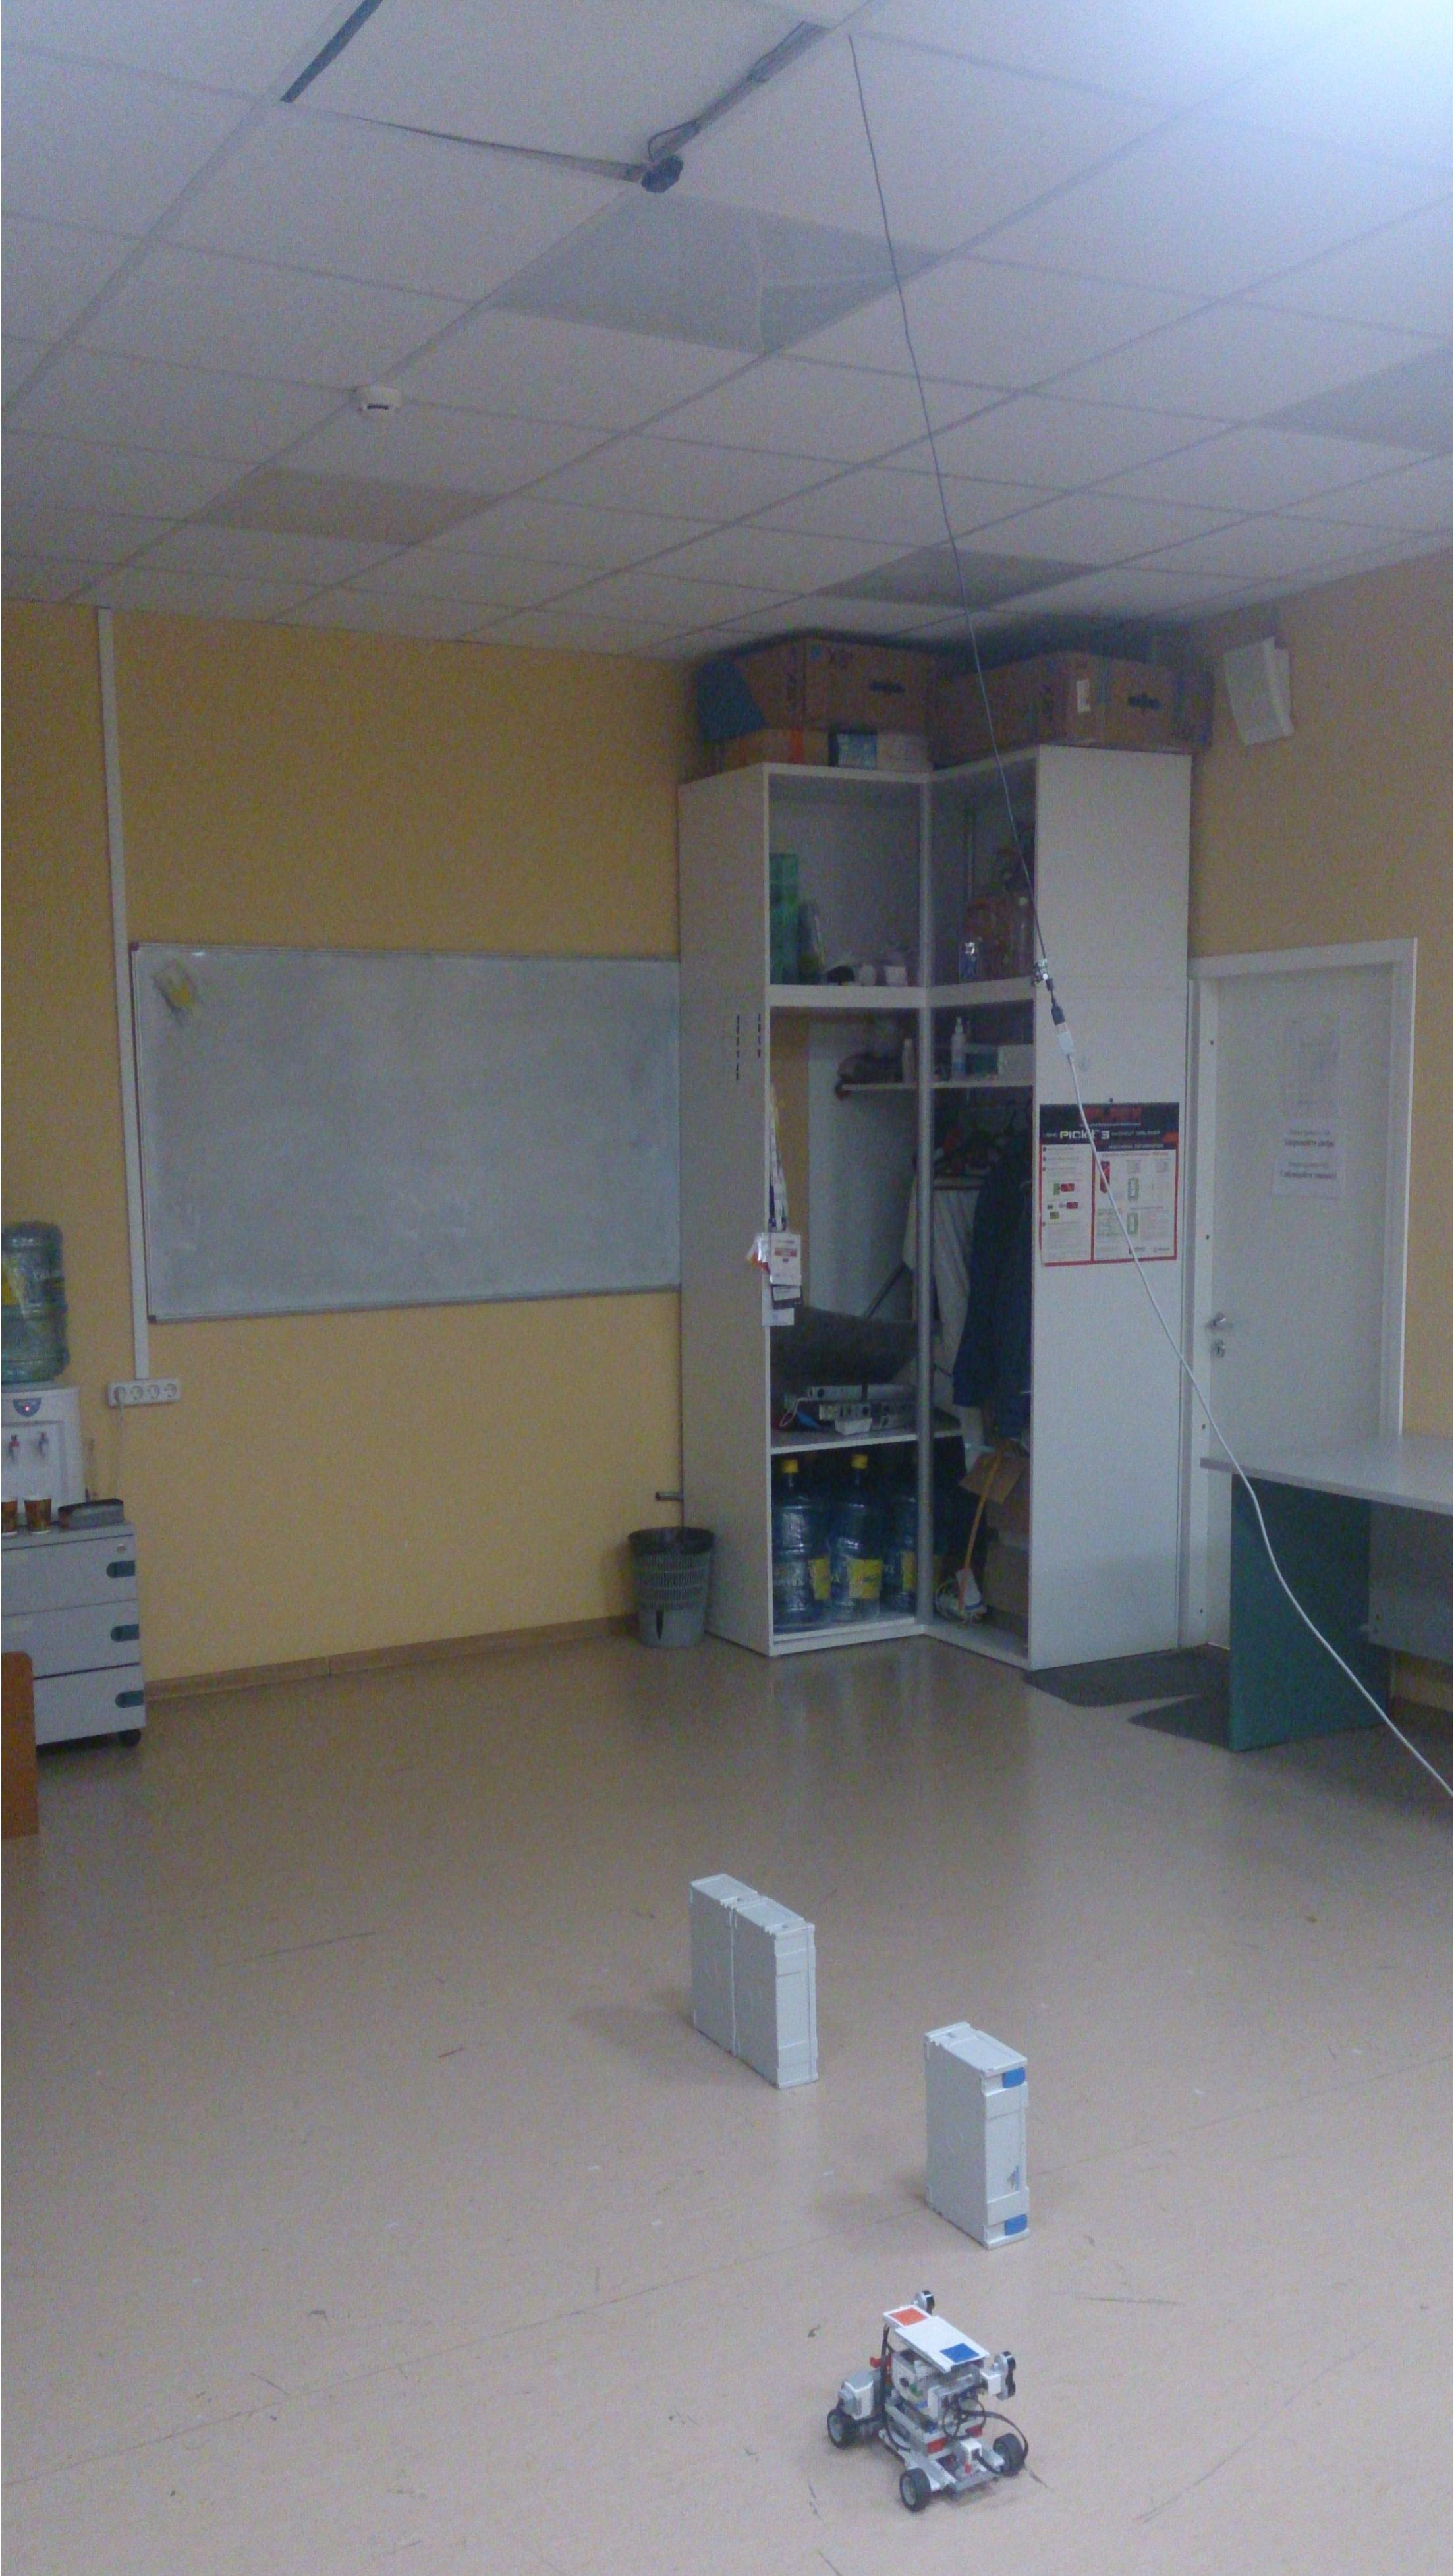
\includegraphics[width= 0.5\textwidth, draft]{test_zone_gen_view.jpg}
    \caption{Общий вид зоны проведения экспериментов.}
    \label{img_test_zone_gen_view}
\end{figure}

Для ее решения авторам пришлось проработать следующие технические вопросы:
\begin{itemize}
    \item создание упомянутого робота из конструктора LEGO Mindstorms EV3;
    \item подбор для него датчиков и программная реализация алгоритмов обработки поступающей с них информации;
    \item проектирование системы управления движением робота;
    \item создание алгоритма картирования парковочного места и его окрестностей.
\end{itemize}
Описанию их ключевых моментов и посвящена основная часть этого документа.


\newpage
\section{Особенности строения робота}
Текст


\newpage
\section{Управление движением робота}
Текст


\newpage
\section{Поиск парковочного места}
Текст


\newpage
\section{Планирование траекторий движения}
Текст


\newpage
\section*{Заключение}
\addcontentsline{toc}{section}{Заключение}
Текст